\apendice{Documentación de usuario}

\section{Introducción}
Esta sección tiene como objetivo proporcionar a los usuarios las instrucciones necesarias para instalar, configurar y utilizar la aplicación Eco City Tours. Este manual está dirigido a usuarios finales interesados en explorar ciudades de manera sostenible, sin necesidad de conocimientos técnicos avanzados.
En primer lugar, se describirán los requisitos mínimos necesarios para ejecutar la aplicación. A continuación, se detallarán los pasos necesarios para instalarla. Finalmente, se presentará una guía práctica para que el usuario pueda aprovechar todas las funcionalidades que ofrece la aplicación.
\section{Requisitos de usuarios}
Para garantizar el correcto funcionamiento de \textbf{Eco City Tours}, el dispositivo debe cumplir con los siguientes requisitos:

\subsection*{Requisitos del Sistema Operativo}
\begin{itemize}
	\item \textbf{Versión mínima de Android:} 6.0 (API 23, Marshmallow).
	\item \textbf{Versión objetivo de Android:} 14 (API 34, Upside Down Cake).
	\item La aplicación está optimizada para las características más recientes de Android 14.
\end{itemize}

\subsection*{Permisos Requeridos}
La aplicación solicita ciertos permisos para ofrecer funcionalidades avanzadas, como el acceso a internet y a la ubicación. Sin embargo, los permisos de localización no son necesarios para iniciar la aplicación y se solicitarán al usuario únicamente cuando sean relevantes para la funcionalidad requerida.

\subsection*{Requisitos de Hardware}
\begin{itemize}
	\item Dispositivo con soporte para \textbf{GPS} y ubicación.
	\item Procesador compatible con arquitecturas ARM o x86.
	\item Acceso a Internet mediante Wi-Fi o red móvil.
\end{itemize}

\section{Instalación}

Para instalar la aplicación \textbf{Eco City Tours} en un dispositivo compatible, siga los siguientes pasos:

\begin{enumerate}
	\item Acceda al repositorio oficial del proyecto en GitHub utilizando el siguiente enlace: 
	\url{https://github.com/fps1001/TFGII_FPisot/releases}.
	\item Busque la \textbf{versión más reciente} de las releases disponibles. Asegúrese de seleccionar la versión adecuada para su dispositivo.
	\item Descargue el archivo \texttt{.apk} correspondiente a esa versión.
	\item Una vez descargado, abra el archivo en su dispositivo móvil para iniciar el proceso de instalación.
	\item Si es la primera vez que instala una aplicación fuera de Google Play Store, es posible que deba habilitar la opción de \textbf{Permitir aplicaciones de fuentes desconocidas} en los ajustes de seguridad de su dispositivo.
	\item Siga las instrucciones que aparecen en pantalla para completar la instalación.
\end{enumerate}

Una vez instalado, la aplicación estará lista para ser configurada y utilizada según las indicaciones del presente manual.

\section{Manual del Usuario}
A continuación, se describen todas las operaciones que puede realizar un usuario de \textbf{Eco City Tours}, explicando todas las funcionalidades de la aplicación, así como los pasos necesarios para utilizarlas de manera efectiva.

\subsection{Habilitar el permiso de uso de GPS}
\begin{figure}[h!]
	\centering
	\begin{tabular}{m{0.4\textwidth} m{0.55\textwidth}}
		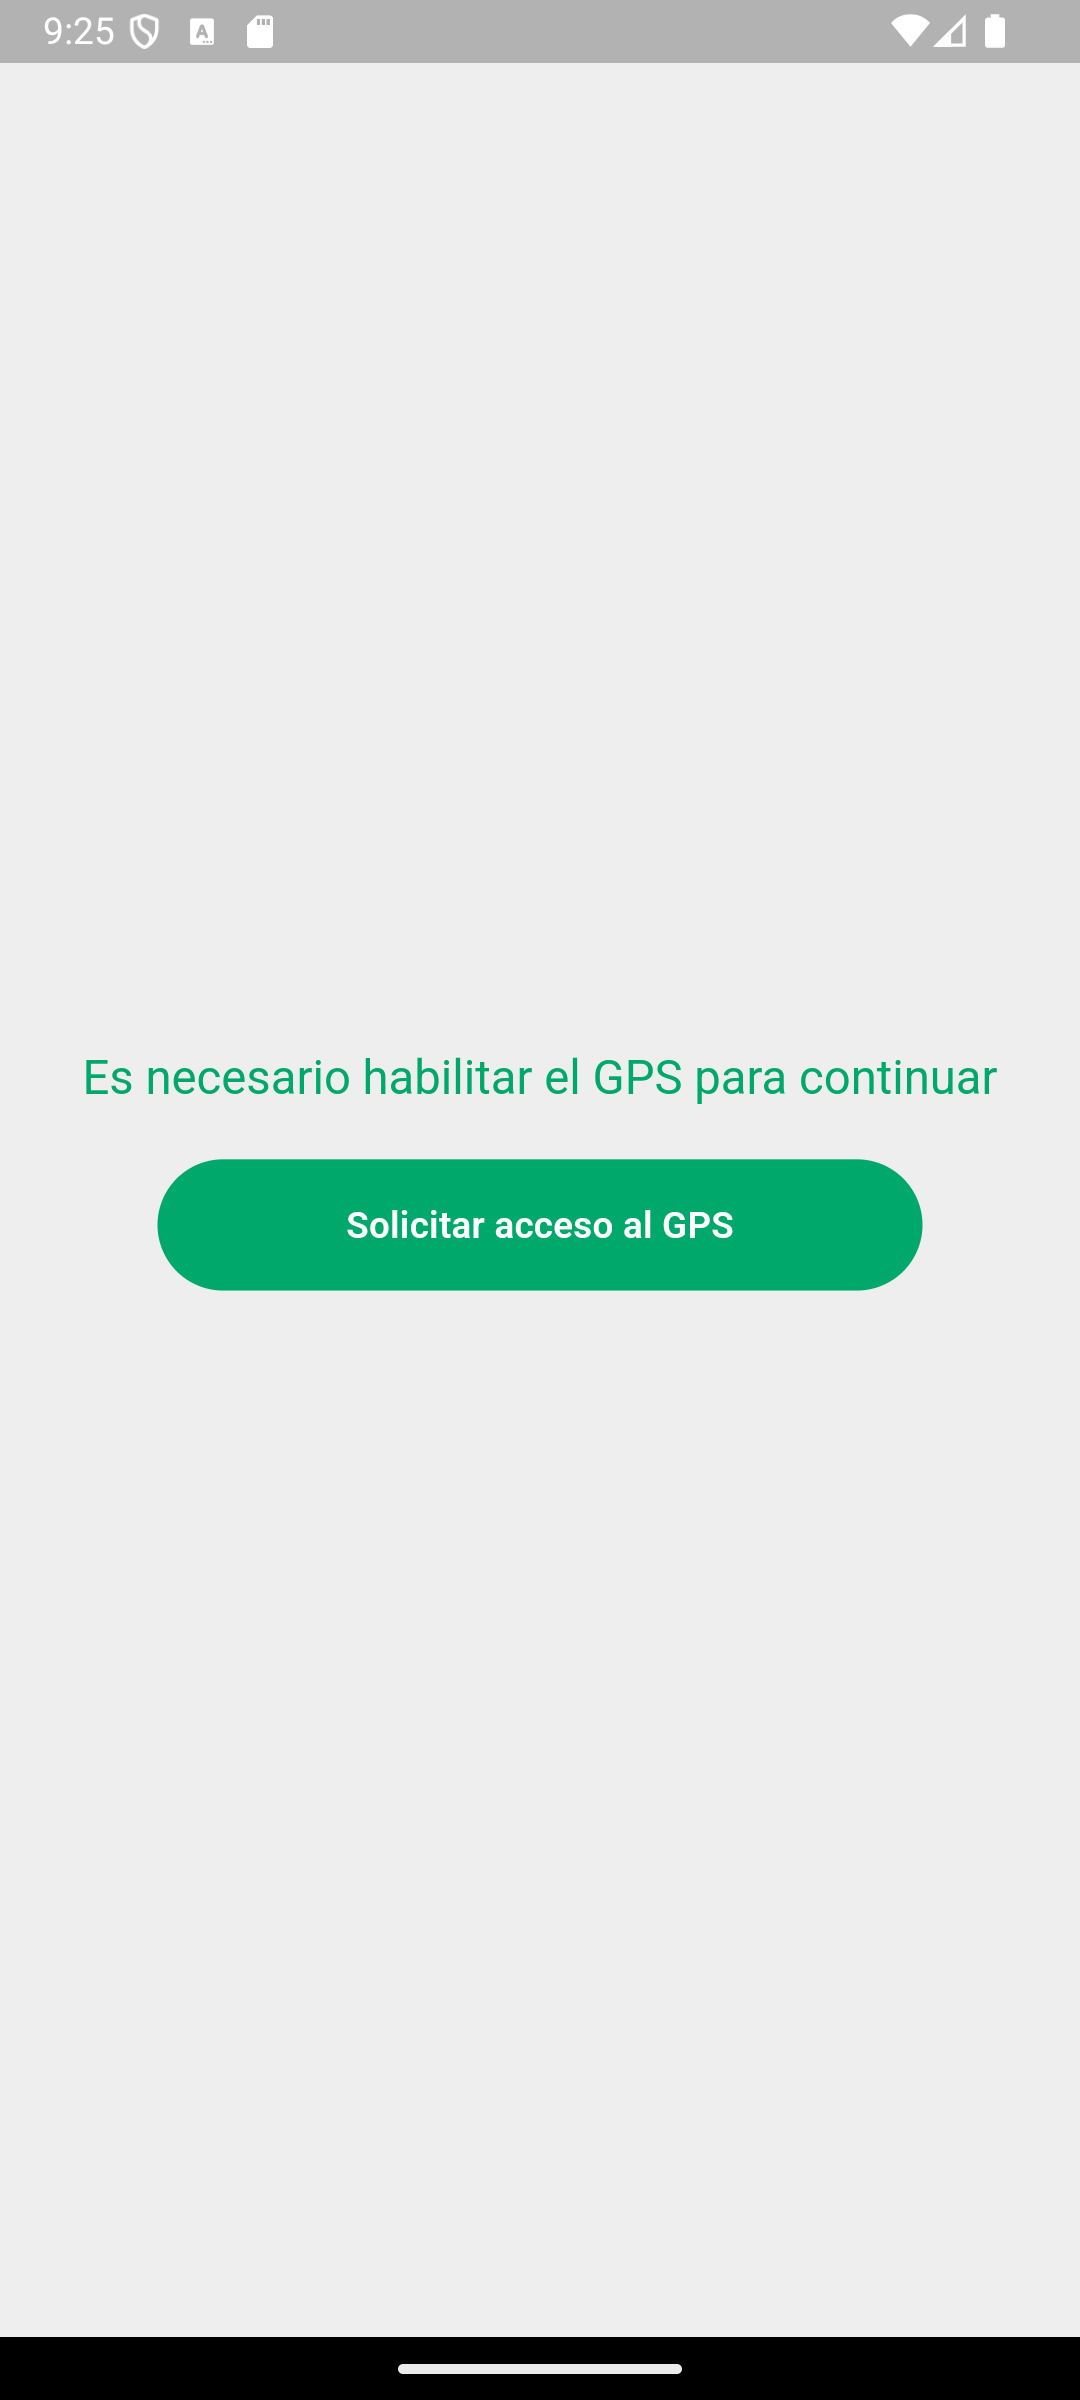
\includegraphics[width=1\linewidth]{E1-habilitar-gps} & 
		\vspace{-10pt}
		
			La primera acción que debe realizar el usuario al iniciar la aplicación es habilitar el permiso de uso de GPS. Esto permite que la aplicación acceda a la ubicación del dispositivo para calcular rutas y mostrar información relevante.
			\textbf{Pasos a seguir:}
			\begin{enumerate}
				\item Al abrir la aplicación por primera vez, aparecerá la pantalla mostrada en la Figura~\ref{fig:habilitarGPS}.
				\item Pulse el botón \textbf{Solicitar acceso al GPS}.
				\item Conceda el permiso solicitado en la ventana emergente.
			\end{enumerate}		
	\end{tabular}
	\caption{Habilitar el permiso de uso de GPS}
	\label{fig:habilitarGPS}
\end{figure}
\newpage
\subsection{Seleccionar opciones de Eco City Tour}
\begin{figure}[h!]
	\centering
	\begin{tabular}{m{0.4\textwidth} m{0.55\textwidth}}
		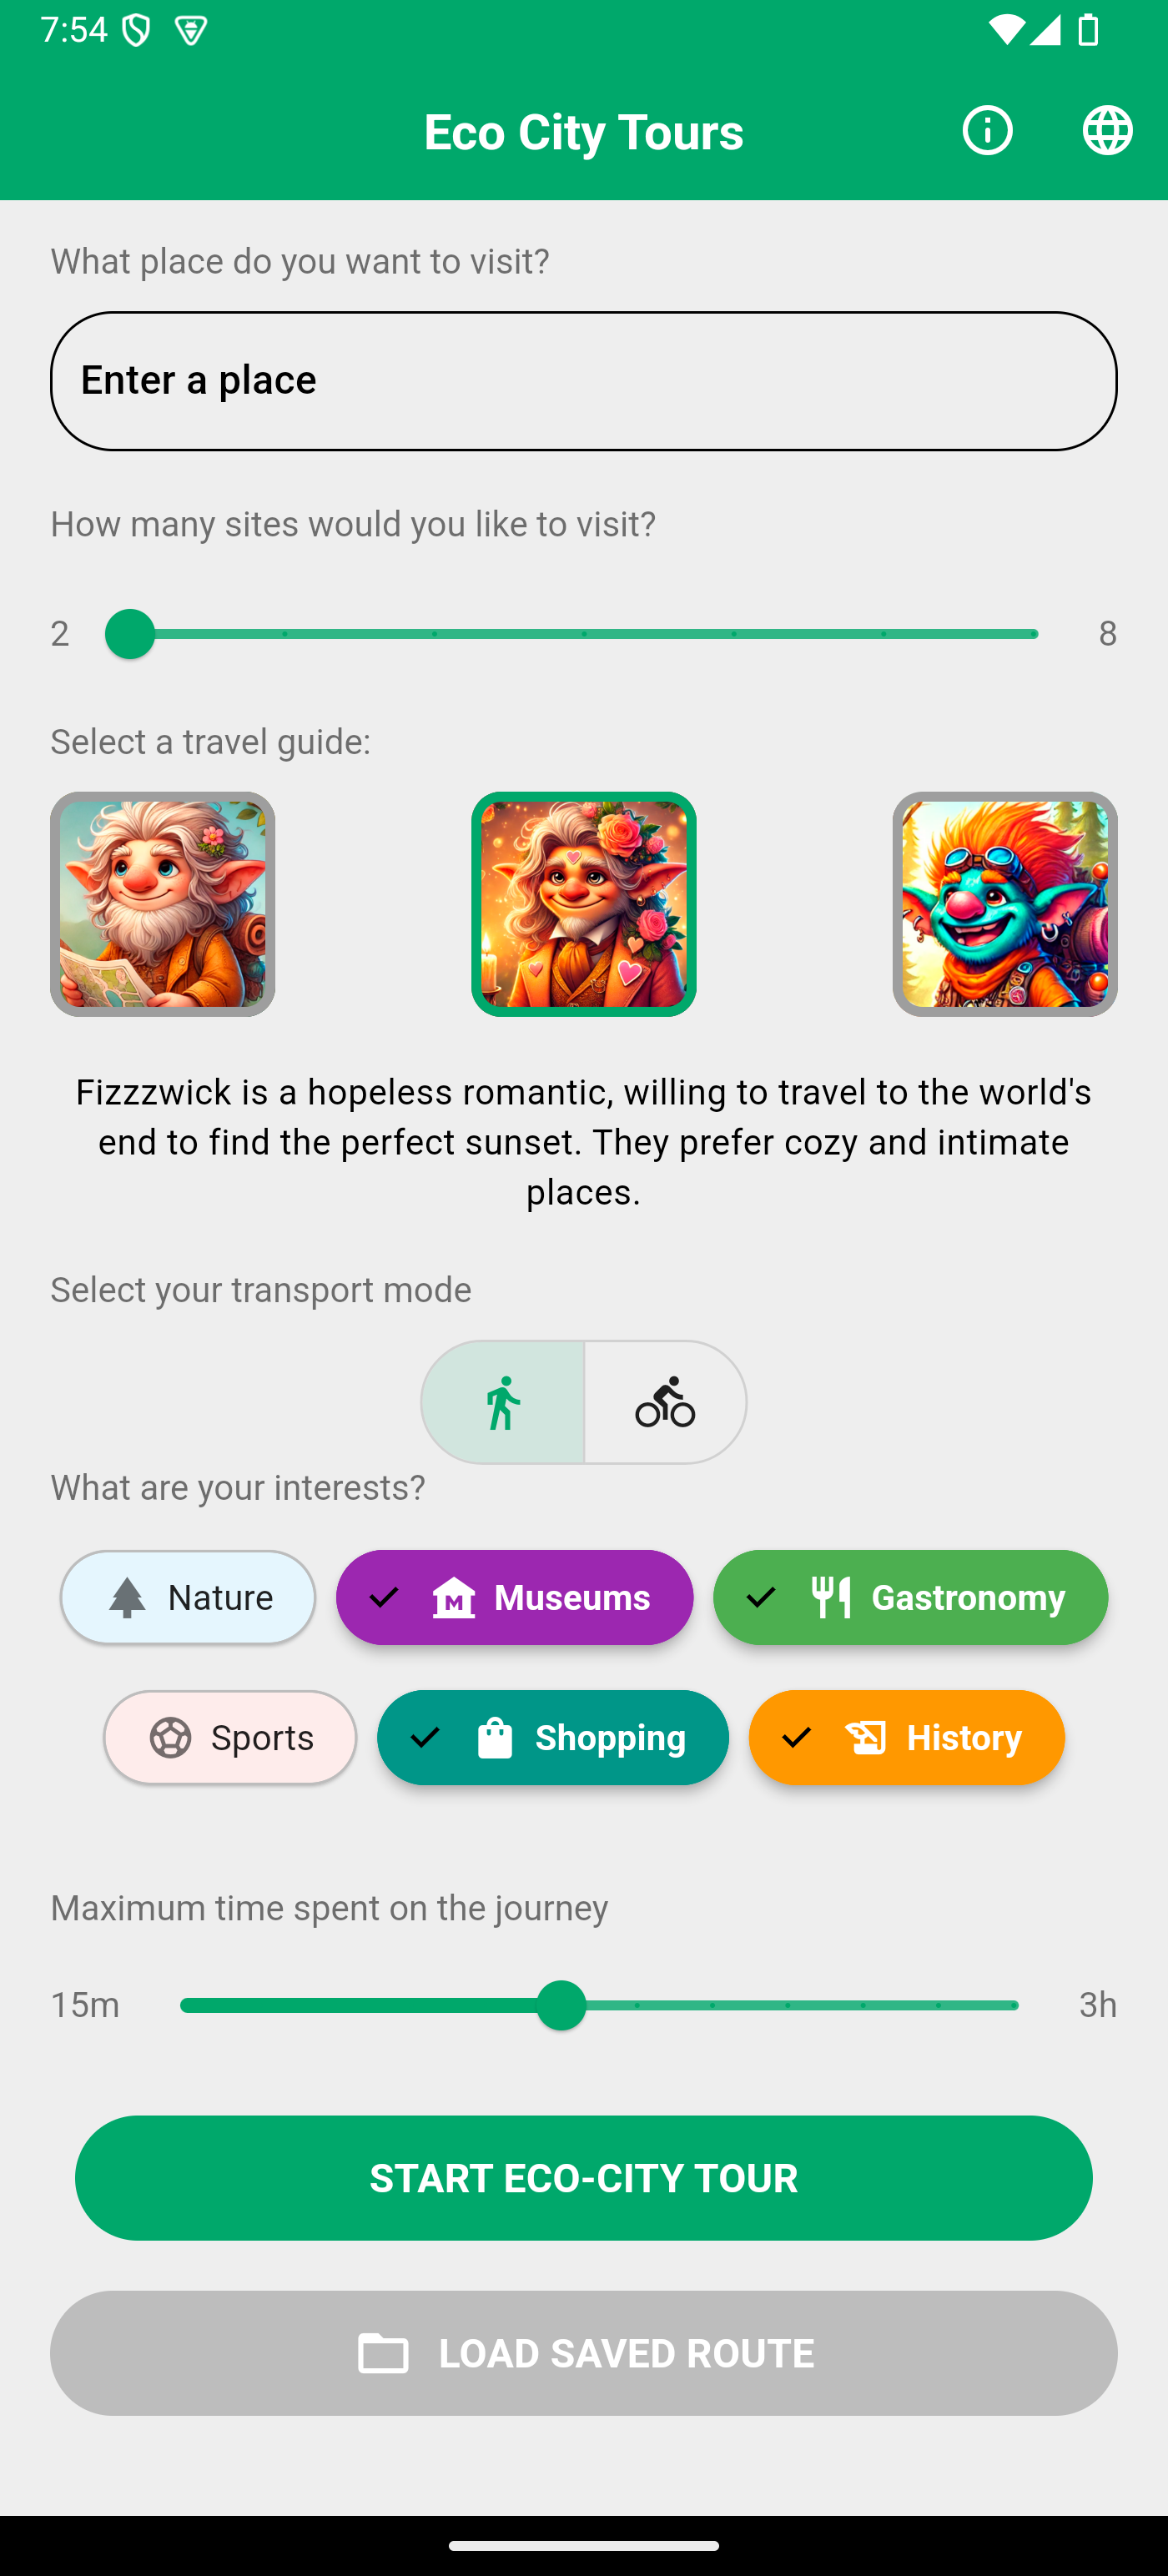
\includegraphics[width=0.6\linewidth]{E2-selection-tour-screen} &		
		
		La primera acción que debe realizar el usuario al iniciar la aplicación es habilitar el permiso de uso de GPS. Esto permite que la aplicación acceda a la ubicación del dispositivo para calcular rutas y mostrar información relevante.
		\textbf{Pasos a seguir:}
		\begin{enumerate}
			\item Al abrir la aplicación por primera vez, aparecerá la pantalla mostrada en la Figura~\ref{fig:selectionTourScreen}.
			\item Pulse el botón \textbf{Solicitar acceso al GPS}.
			\item Conceda el permiso solicitado en la ventana emergente.
		\end{enumerate}		
	\end{tabular}
	\caption{Pantalla de configuración de Eco City Tour}
	\label{fig:selectionTourScreen}
\end{figure}
\subsection{Visualizar Eco City Tour generado}
\begin{figure}[h!]
	\centering
	\begin{tabular}{m{0.4\textwidth} m{0.55\textwidth}}
		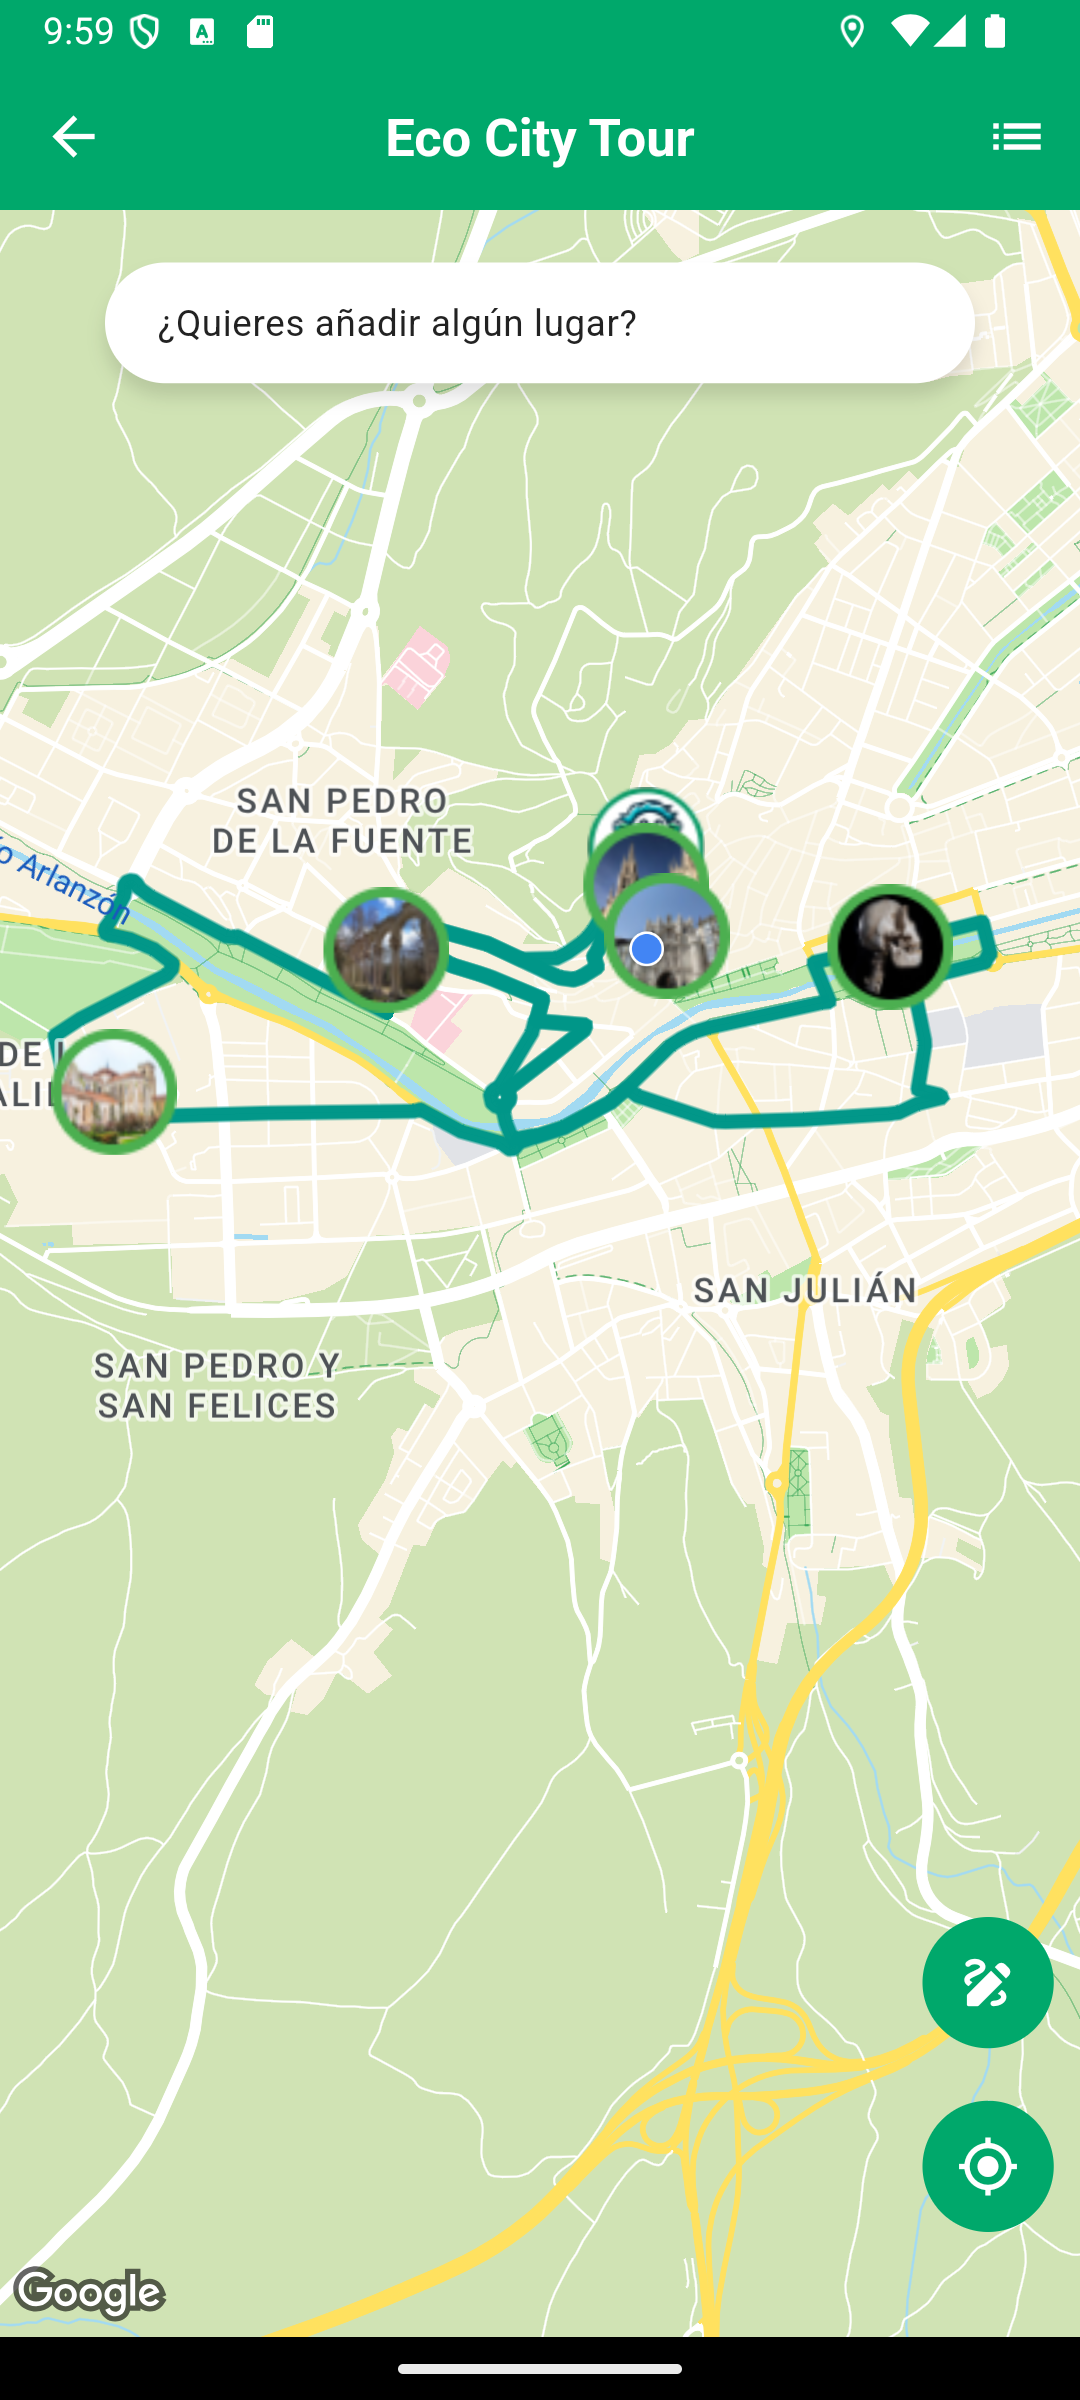
\includegraphics[width=0.6\linewidth]{E3-map-screen} & 
		\vspace{-10pt}
		
		La primera acción que debe realizar el usuario al iniciar la aplicación es habilitar el permiso de uso de GPS. Esto permite que la aplicación acceda a la ubicación del dispositivo para calcular rutas y mostrar información relevante.
		\textbf{Pasos a seguir:}
		\begin{enumerate}
			\item Al abrir la aplicación por primera vez, aparecerá la pantalla mostrada en la .
			\item Pulse el botón \textbf{Solicitar acceso al GPS}.
			\item Conceda el permiso solicitado en la ventana emergente.
		\end{enumerate}		
	\end{tabular}
	\caption{Pantalla de navegación de mapa}
	\label{fig:navegacionMapa}
\end{figure}

\subsection{Buscar y añadir un \acrlong{pdi} al Eco City Tour}
\begin{figure}[h!]
	\centering
	\begin{tabular}{m{0.4\textwidth} m{0.55\textwidth}}
		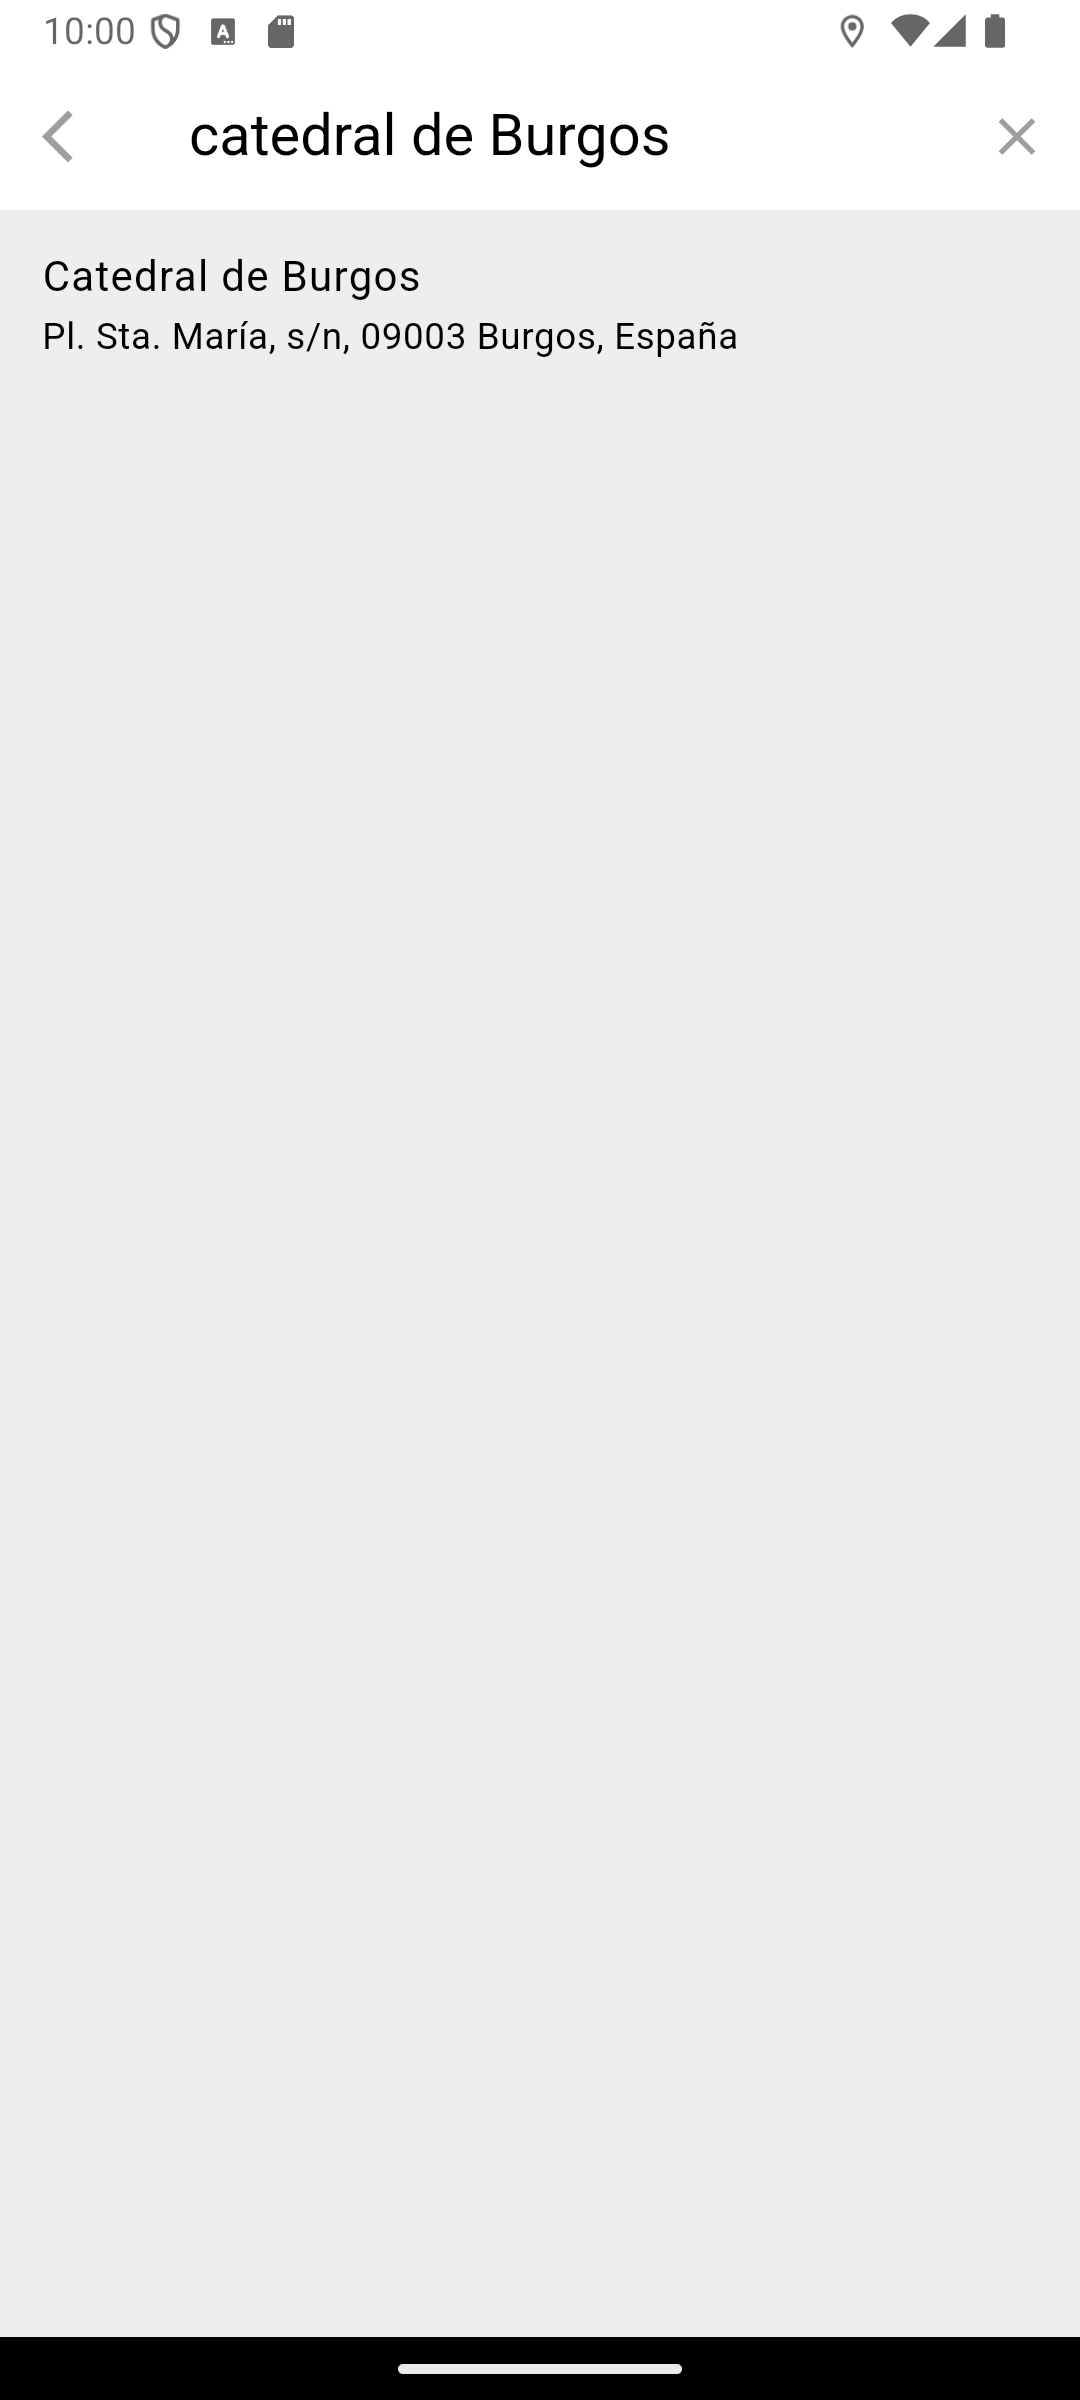
\includegraphics[width=0.6\linewidth]{E4-search-bar} & 
		\vspace{-10pt}
		
		La primera acción que debe realizar el usuario al iniciar la aplicación es habilitar el permiso de uso de GPS. Esto permite que la aplicación acceda a la ubicación del dispositivo para calcular rutas y mostrar información relevante.
		\textbf{Pasos a seguir:}
		\begin{enumerate}
			\item Al abrir la aplicación por primera vez, aparecerá la pantalla mostrada en la Figura~\ref{fig:busquedaPDI}.
			\item Pulse el botón \textbf{Solicitar acceso al GPS}.
			\item Conceda el permiso solicitado en la ventana emergente.
		\end{enumerate}		
	\end{tabular}
	\caption{Búsqueda de \acrshort{pdi}}
	\label{fig:busquedaPDI}
\end{figure}

\subsection{Conocer detalle de \acrshort{pdi}}
\begin{figure}[h!]
	\centering
	\begin{tabular}{m{0.4\textwidth} m{0.55\textwidth}}
		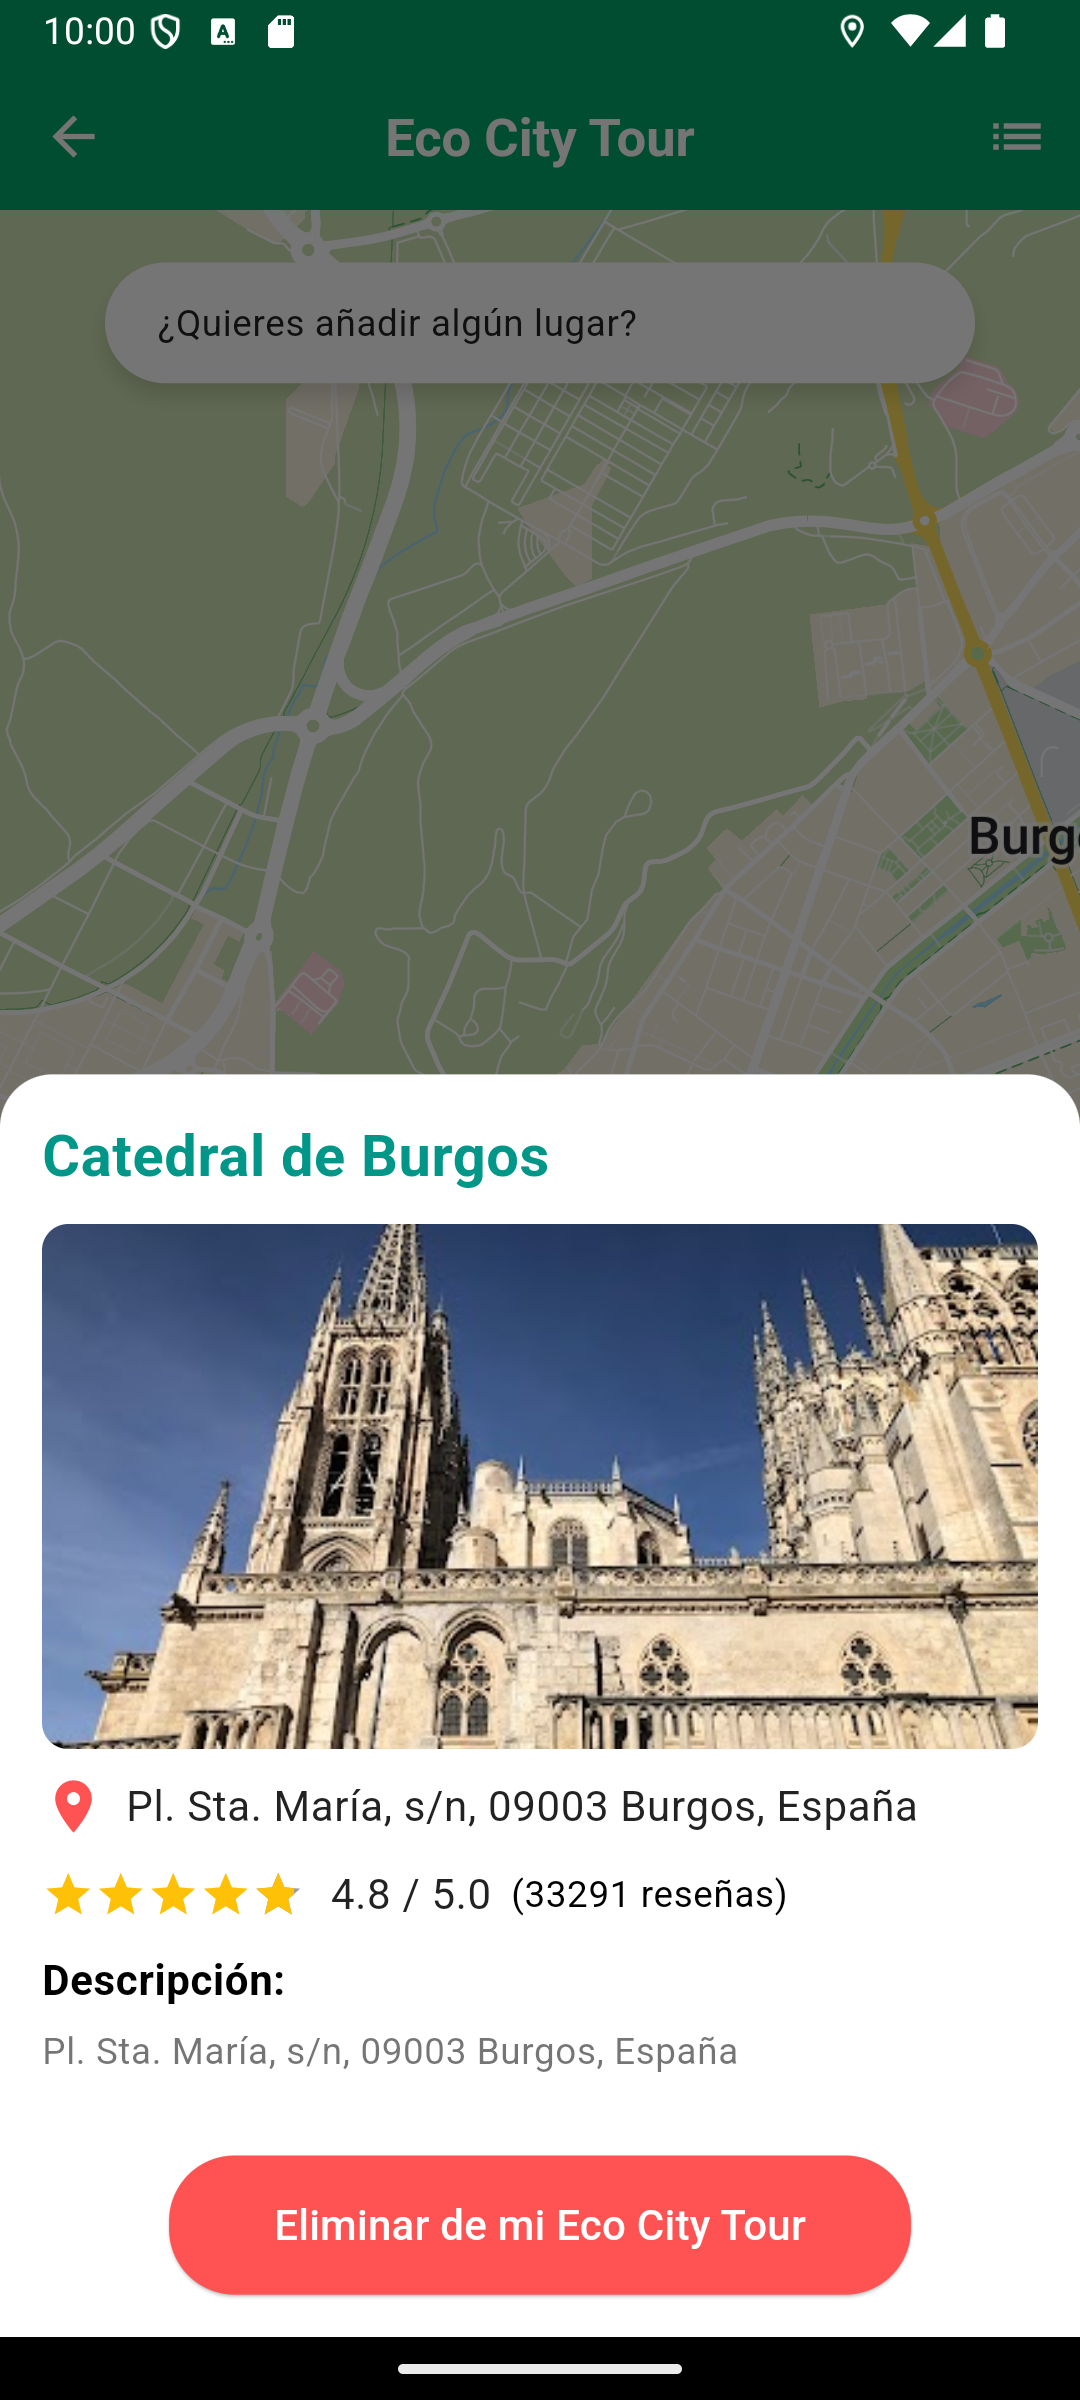
\includegraphics[width=0.6\linewidth]{E5-PDI-detalle} & 
		\vspace{-10pt}
		
		La primera acción que debe realizar el usuario al iniciar la aplicación es habilitar el permiso de uso de GPS. Esto permite que la aplicación acceda a la ubicación del dispositivo para calcular rutas y mostrar información relevante.
		\textbf{Pasos a seguir:}
		\begin{enumerate}
			\item Al abrir la aplicación por primera vez, aparecerá la pantalla mostrada en la Figura~\ref{fig:detallePDI}.
			\item Pulse el botón \textbf{Solicitar acceso al GPS}.
			\item Conceda el permiso solicitado en la ventana emergente.
		\end{enumerate}		
	\end{tabular}
	\caption{Detalle de \acrshort{pdi}}
	\label{fig:detallePDI}
\end{figure}

\subsection{Resumen de Eco City Tour creado}
\begin{figure}[h!]
	\centering
	\begin{tabular}{m{0.4\textwidth} m{0.55\textwidth}}
		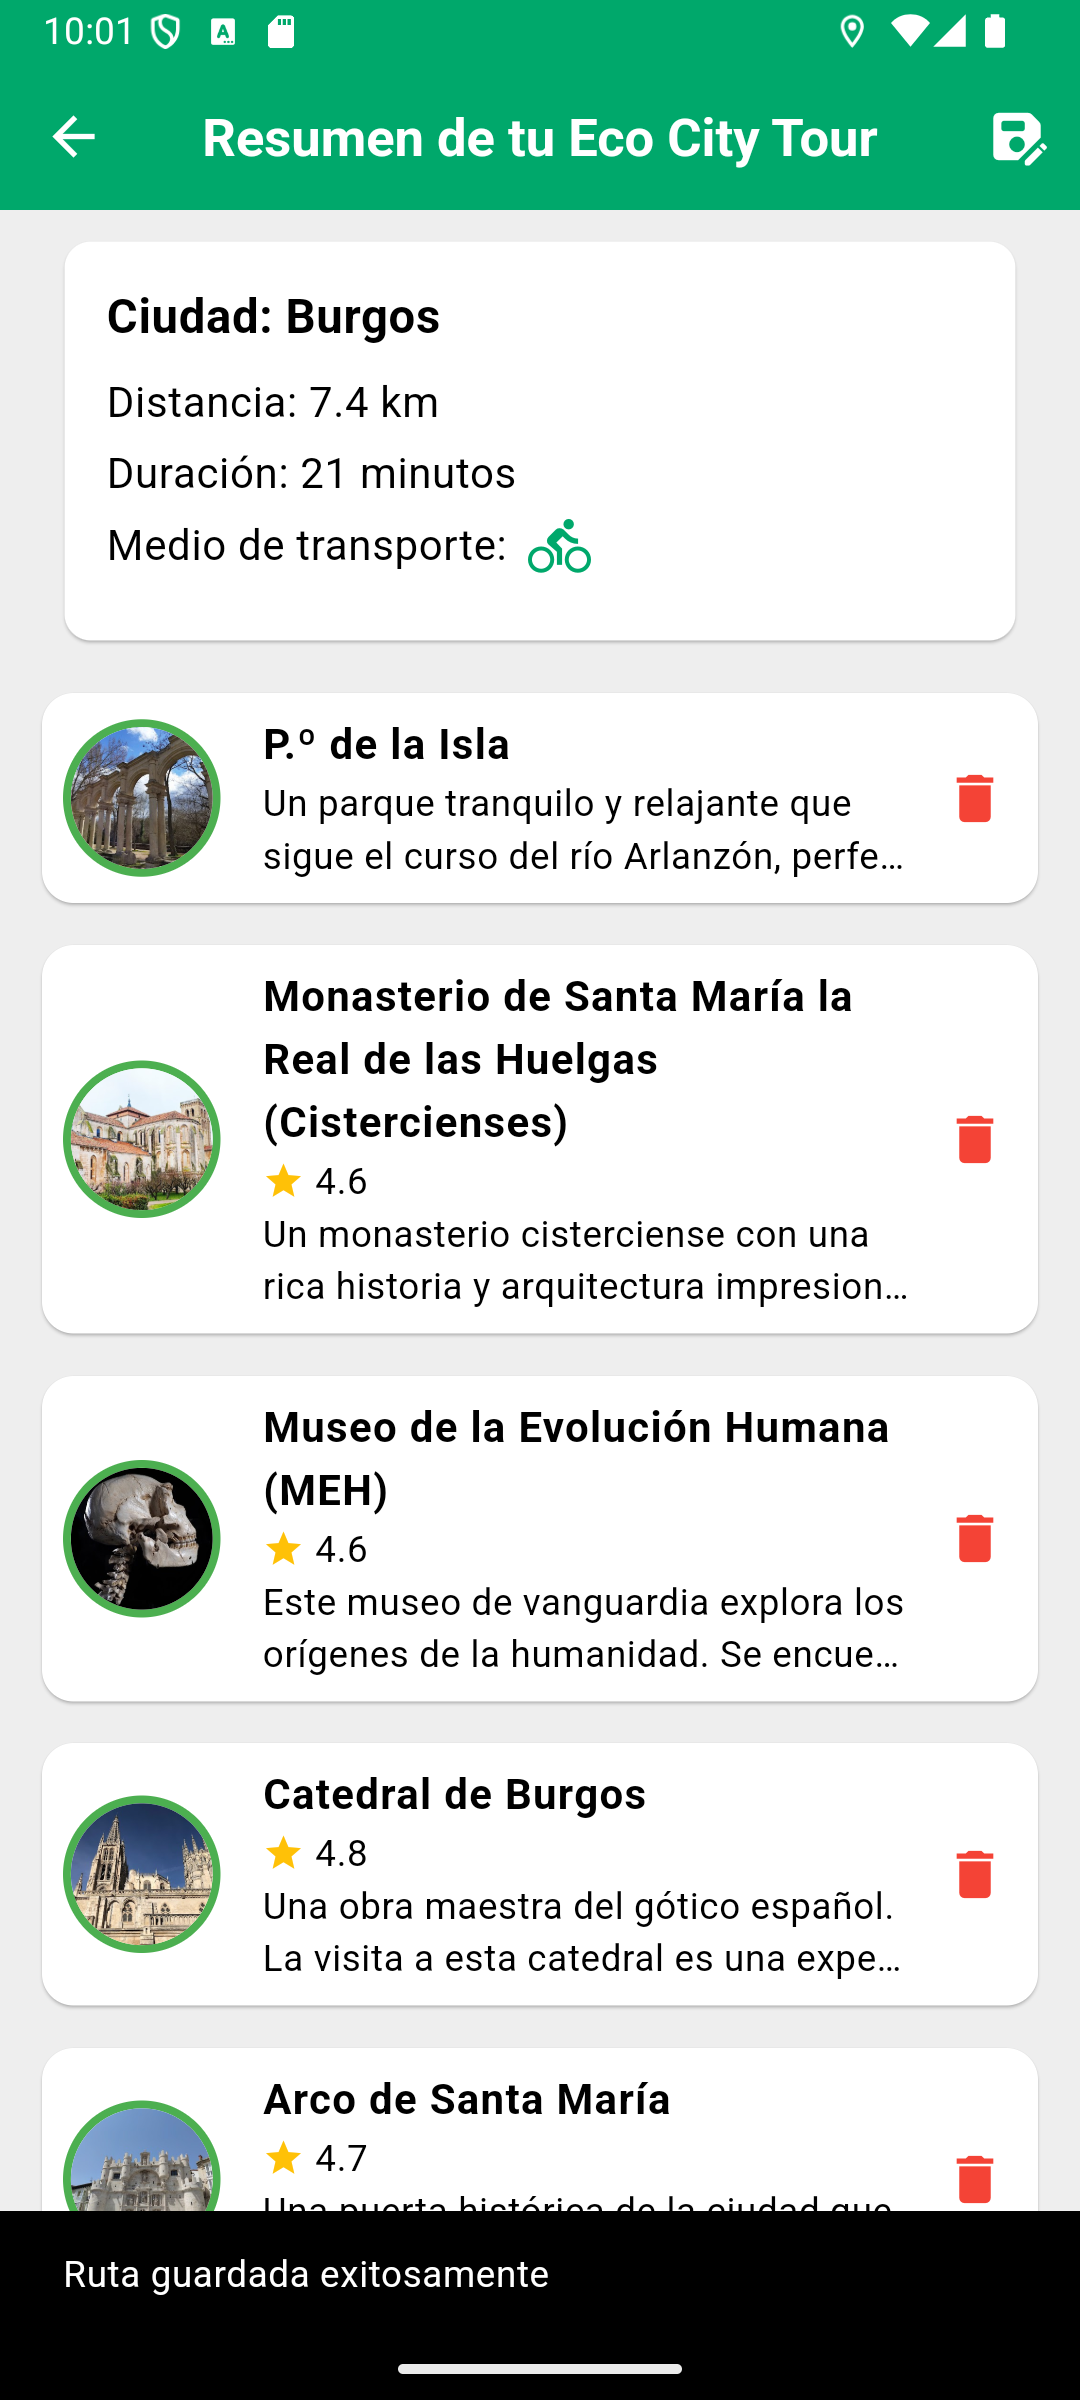
\includegraphics[width=0.6\linewidth]{E6-summary-screen} & 
		\vspace{-10pt}
		
		La primera acción que debe realizar el usuario al iniciar la aplicación es habilitar el permiso de uso de GPS. Esto permite que la aplicación acceda a la ubicación del dispositivo para calcular rutas y mostrar información relevante.
		\textbf{Pasos a seguir:}
		\begin{enumerate}
			\item Al abrir la aplicación por primera vez, aparecerá la pantalla mostrada en la Figura~\ref{fig:resumenECT}.
			\item Pulse el botón \textbf{Solicitar acceso al GPS}.
			\item Conceda el permiso solicitado en la ventana emergente.
		\end{enumerate}		
	\end{tabular}
	\caption{Pantalla de resumen del Eco City Tour}
	\label{fig:resumenECT}
\end{figure}

\subsection{Guardar Eco City Tour}
\begin{figure}[h!]
	\centering
	\begin{tabular}{m{0.4\textwidth} m{0.55\textwidth}}
		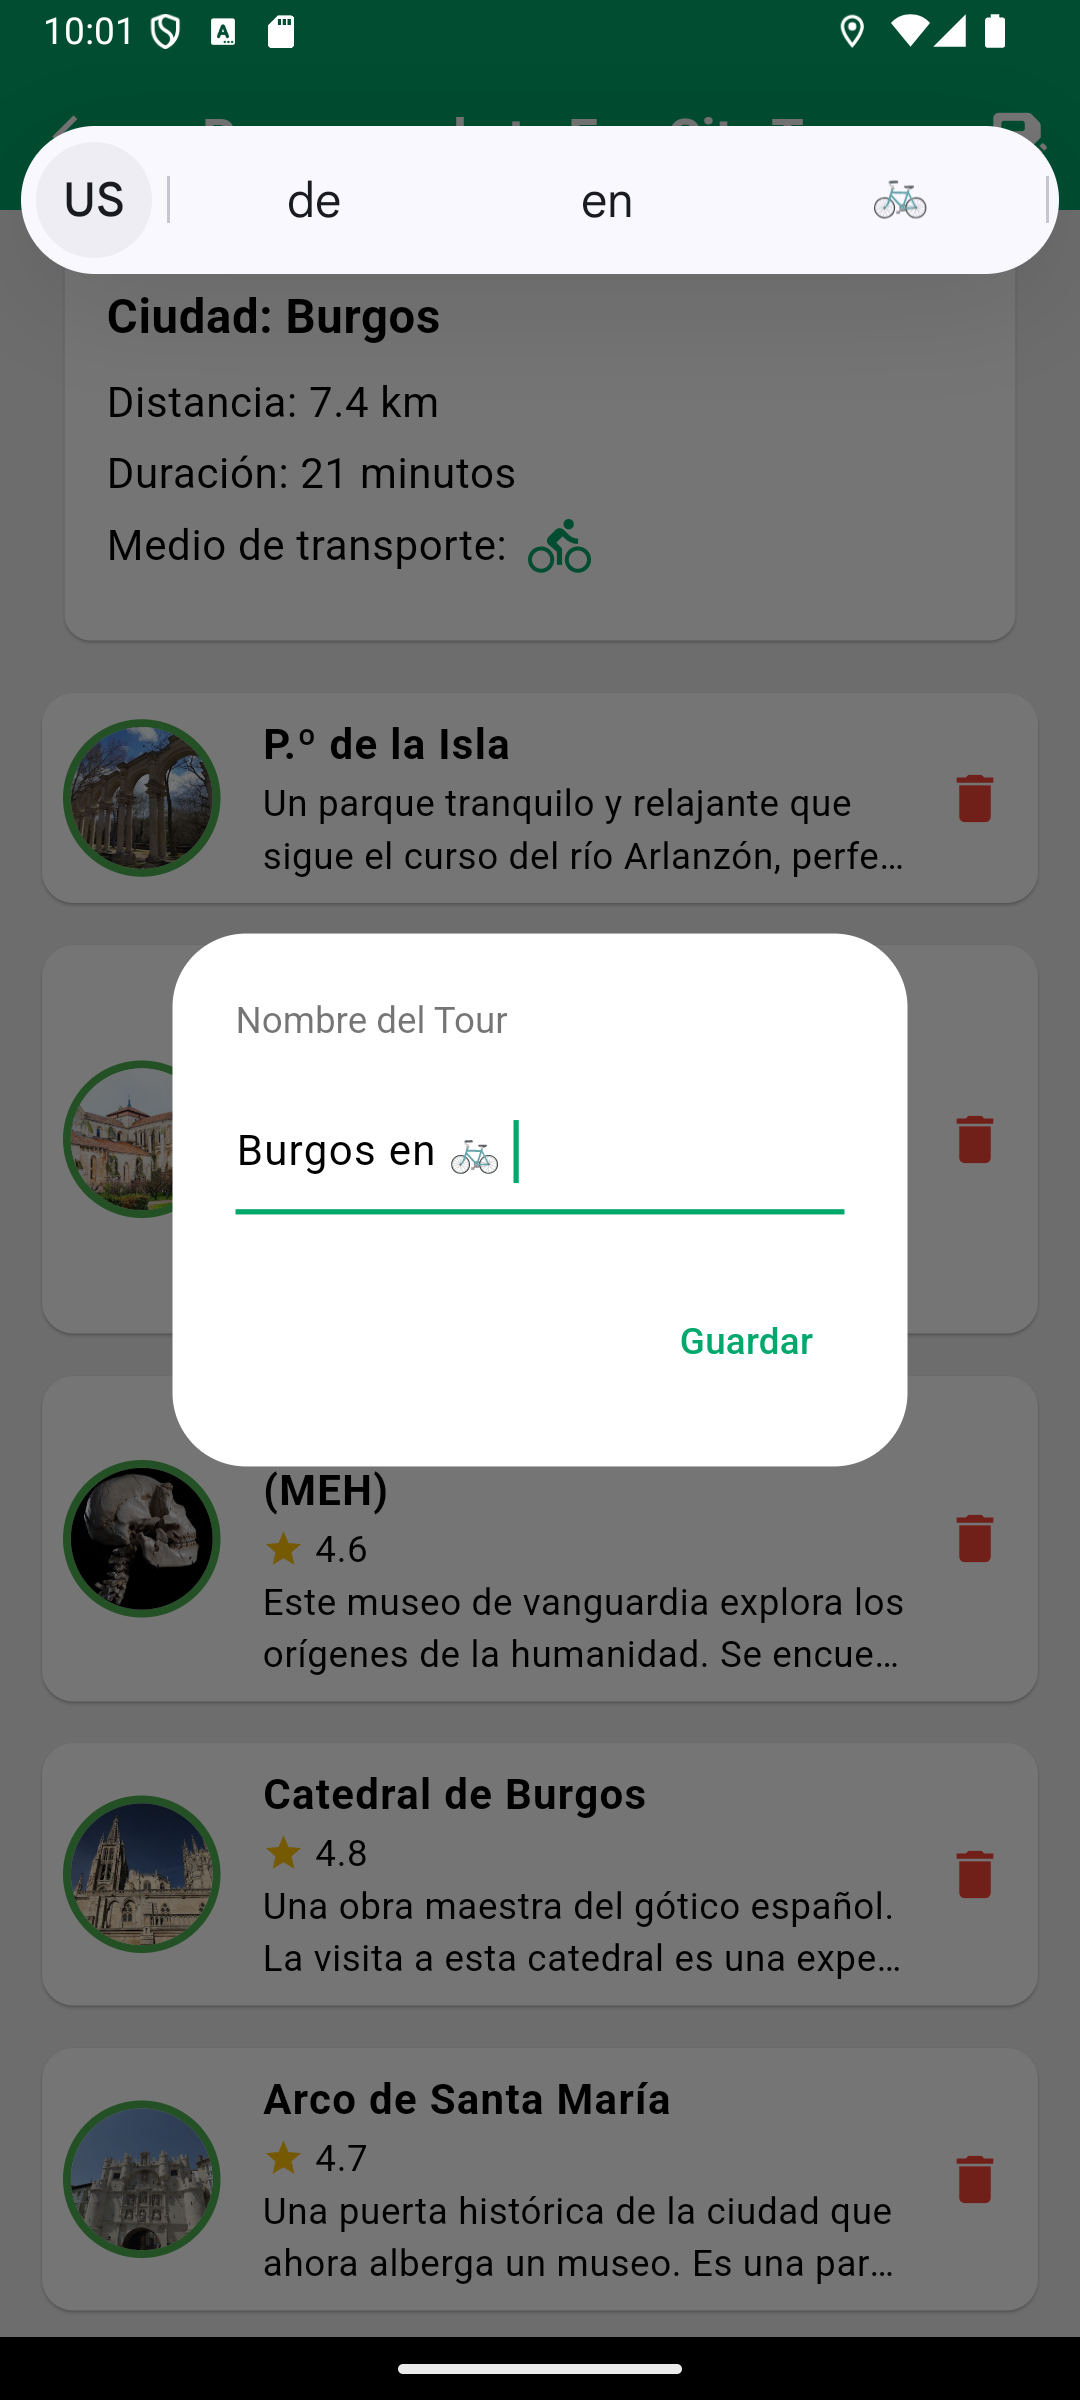
\includegraphics[width=0.6\linewidth]{E7-save-tour} & 
		\vspace{-10pt}
		
		La primera acción que debe realizar el usuario al iniciar la aplicación es habilitar el permiso de uso de GPS. Esto permite que la aplicación acceda a la ubicación del dispositivo para calcular rutas y mostrar información relevante.
		\textbf{Pasos a seguir:}
		\begin{enumerate}
			\item Al abrir la aplicación por primera vez, aparecerá la pantalla mostrada en la Figura~\ref{fig:saveECT}.
			\item Pulse el botón \textbf{Solicitar acceso al GPS}.
			\item Conceda el permiso solicitado en la ventana emergente.
		\end{enumerate}		
	\end{tabular}
	\caption{Pantalla de guardado del Eco City Tour}
	\label{fig:saveECT}
\end{figure}

\subsection{Cargar Eco City Tour}
\begin{figure}[h!]
	\centering
	\begin{tabular}{m{0.4\textwidth} m{0.55\textwidth}}
		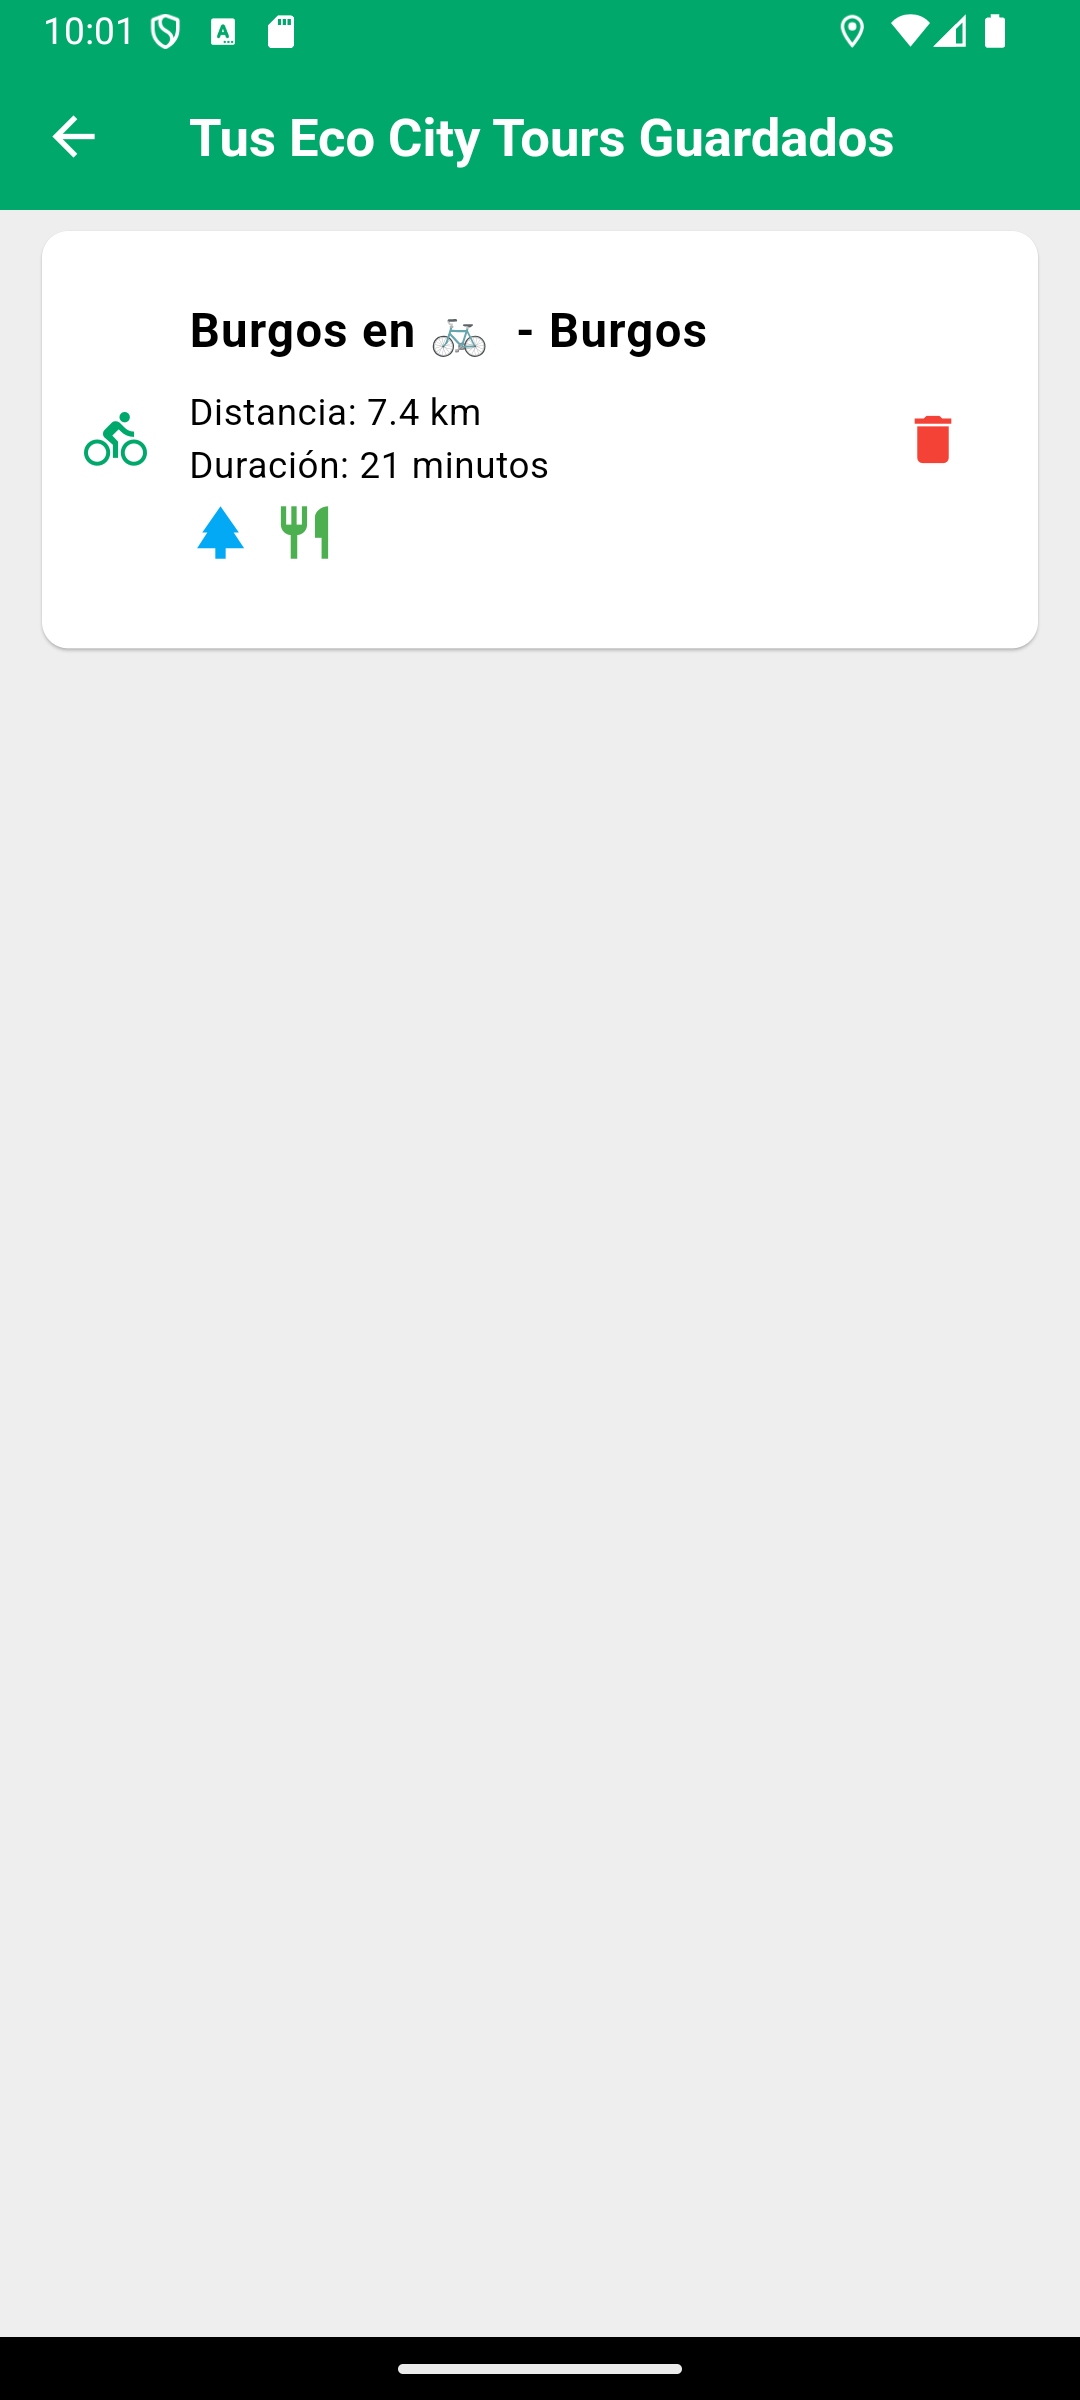
\includegraphics[width=0.6\linewidth]{E8-load-tour} & 
		\vspace{-10pt}
		
		La primera acción que debe realizar el usuario al iniciar la aplicación es habilitar el permiso de uso de GPS. Esto permite que la aplicación acceda a la ubicación del dispositivo para calcular rutas y mostrar información relevante.
		\textbf{Pasos a seguir:}
		\begin{enumerate}
			\item Al abrir la aplicación por primera vez, aparecerá la pantalla mostrada en la Figura~\ref{fig:loadECT}.
			\item Pulse el botón \textbf{Solicitar acceso al GPS}.
			\item Conceda el permiso solicitado en la ventana emergente.
		\end{enumerate}		
	\end{tabular}
	\caption{Pantalla de carga del Eco City Tour}
	\label{fig:loadECT}
\end{figure}

\subsection{Seguimiento en vivo de la posición del usuario}
\begin{figure}[h!]
	\centering
	\begin{tabular}{m{0.4\textwidth} m{0.55\textwidth}}
		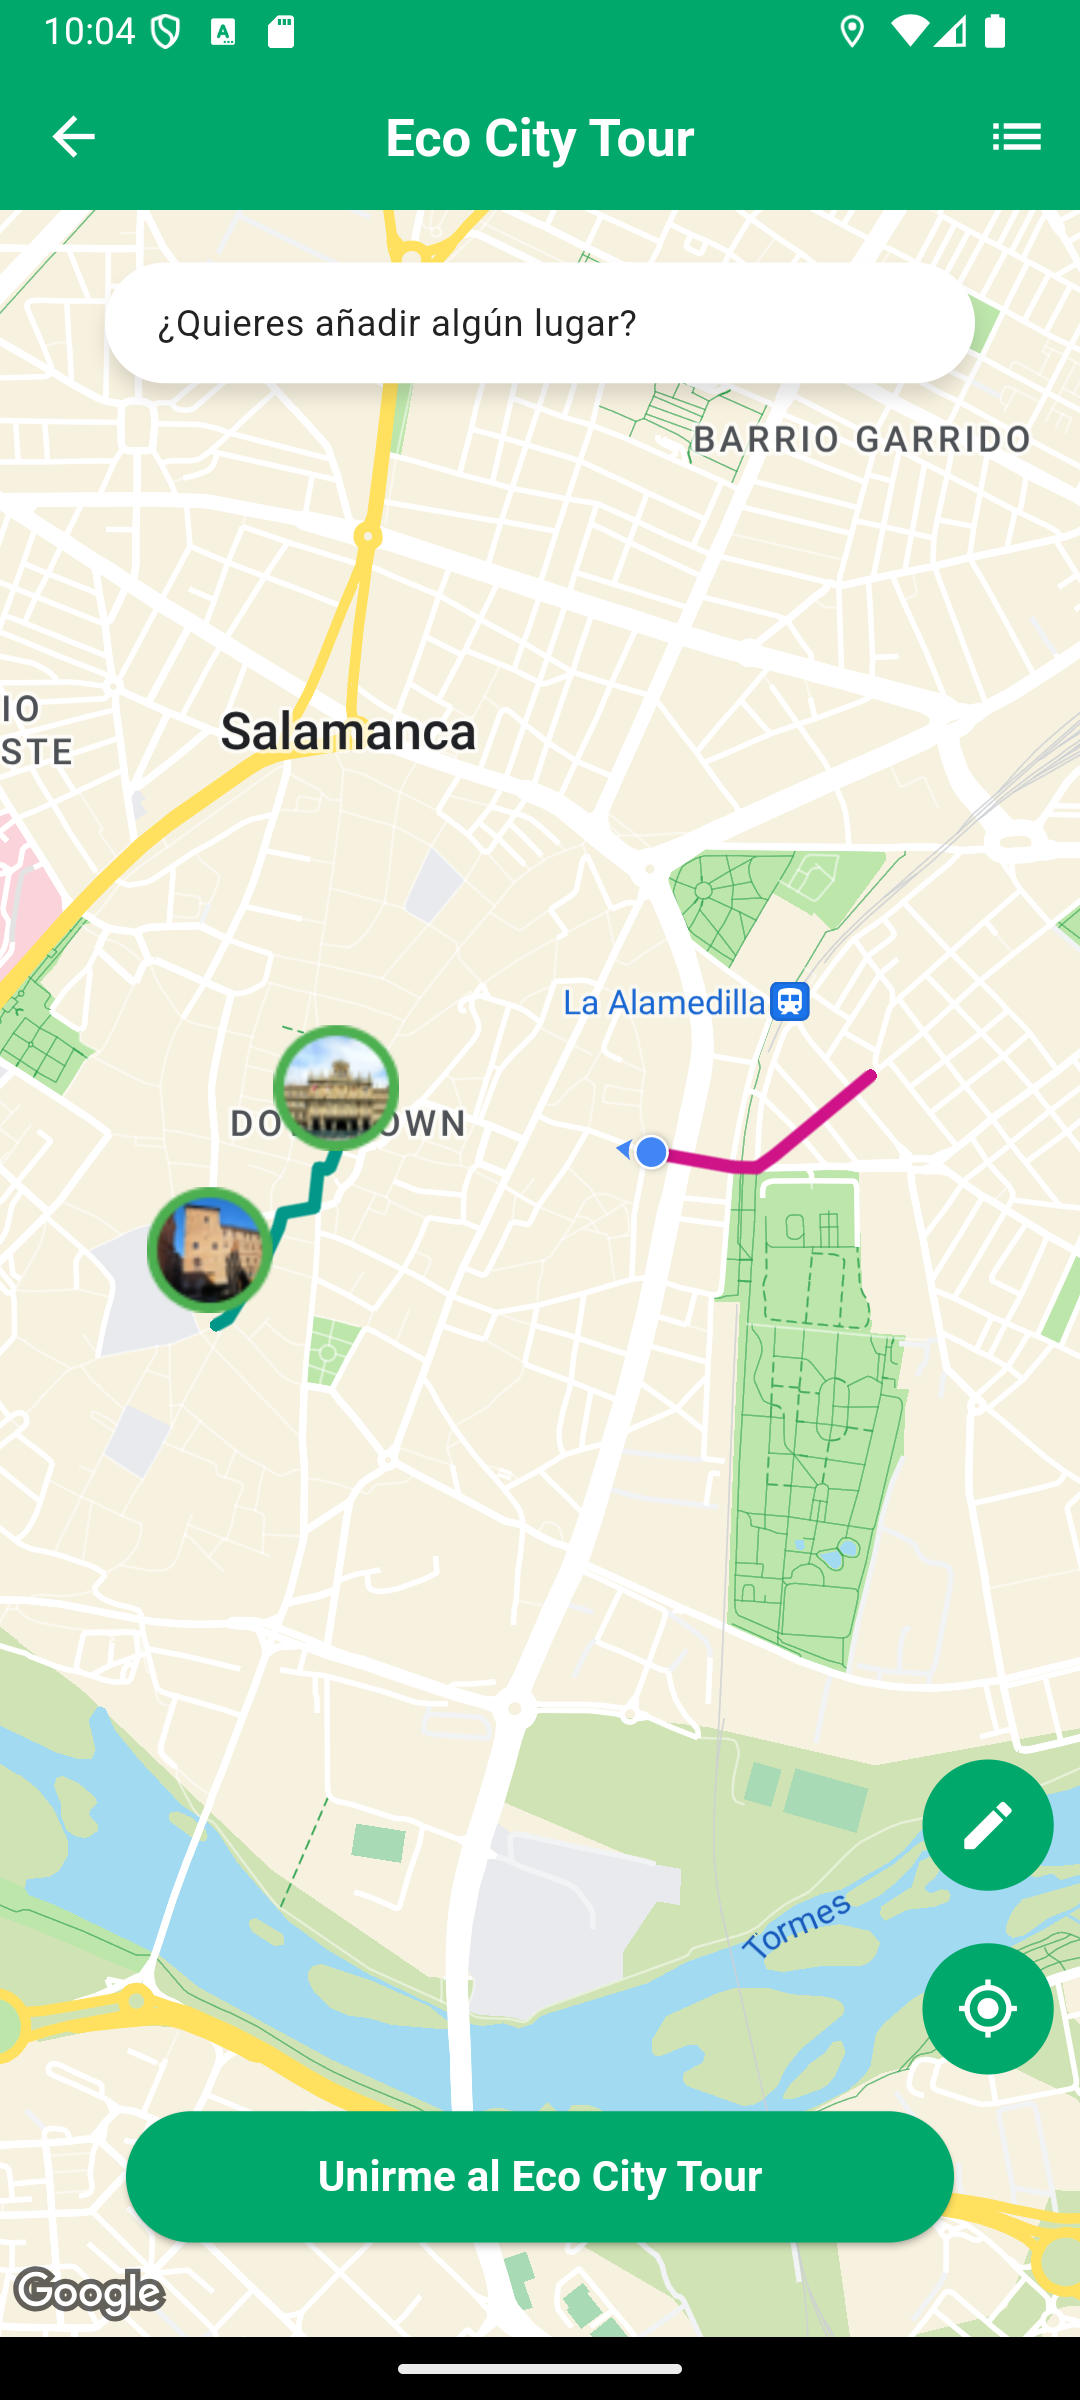
\includegraphics[width=0.6\linewidth]{E9-following-user} & 
		\vspace{-10pt}
		
		La primera acción que debe realizar el usuario al iniciar la aplicación es habilitar el permiso de uso de GPS. Esto permite que la aplicación acceda a la ubicación del dispositivo para calcular rutas y mostrar información relevante.
		\textbf{Pasos a seguir:}
		\begin{enumerate}
			\item Al abrir la aplicación por primera vez, aparecerá la pantalla mostrada en la Figura~\ref{fig:followingUser}.
			\item Pulse el botón \textbf{Solicitar acceso al GPS}.
			\item Conceda el permiso solicitado en la ventana emergente.
		\end{enumerate}		
	\end{tabular}
	\caption{Seguimiento en vivo de la posición del usuario}
	\label{fig:followingUser}
\end{figure}

\subsection{Unirse al Eco City Tour}
\begin{figure}[h!]
	\centering
	\begin{tabular}{m{0.4\textwidth} m{0.55\textwidth}}
		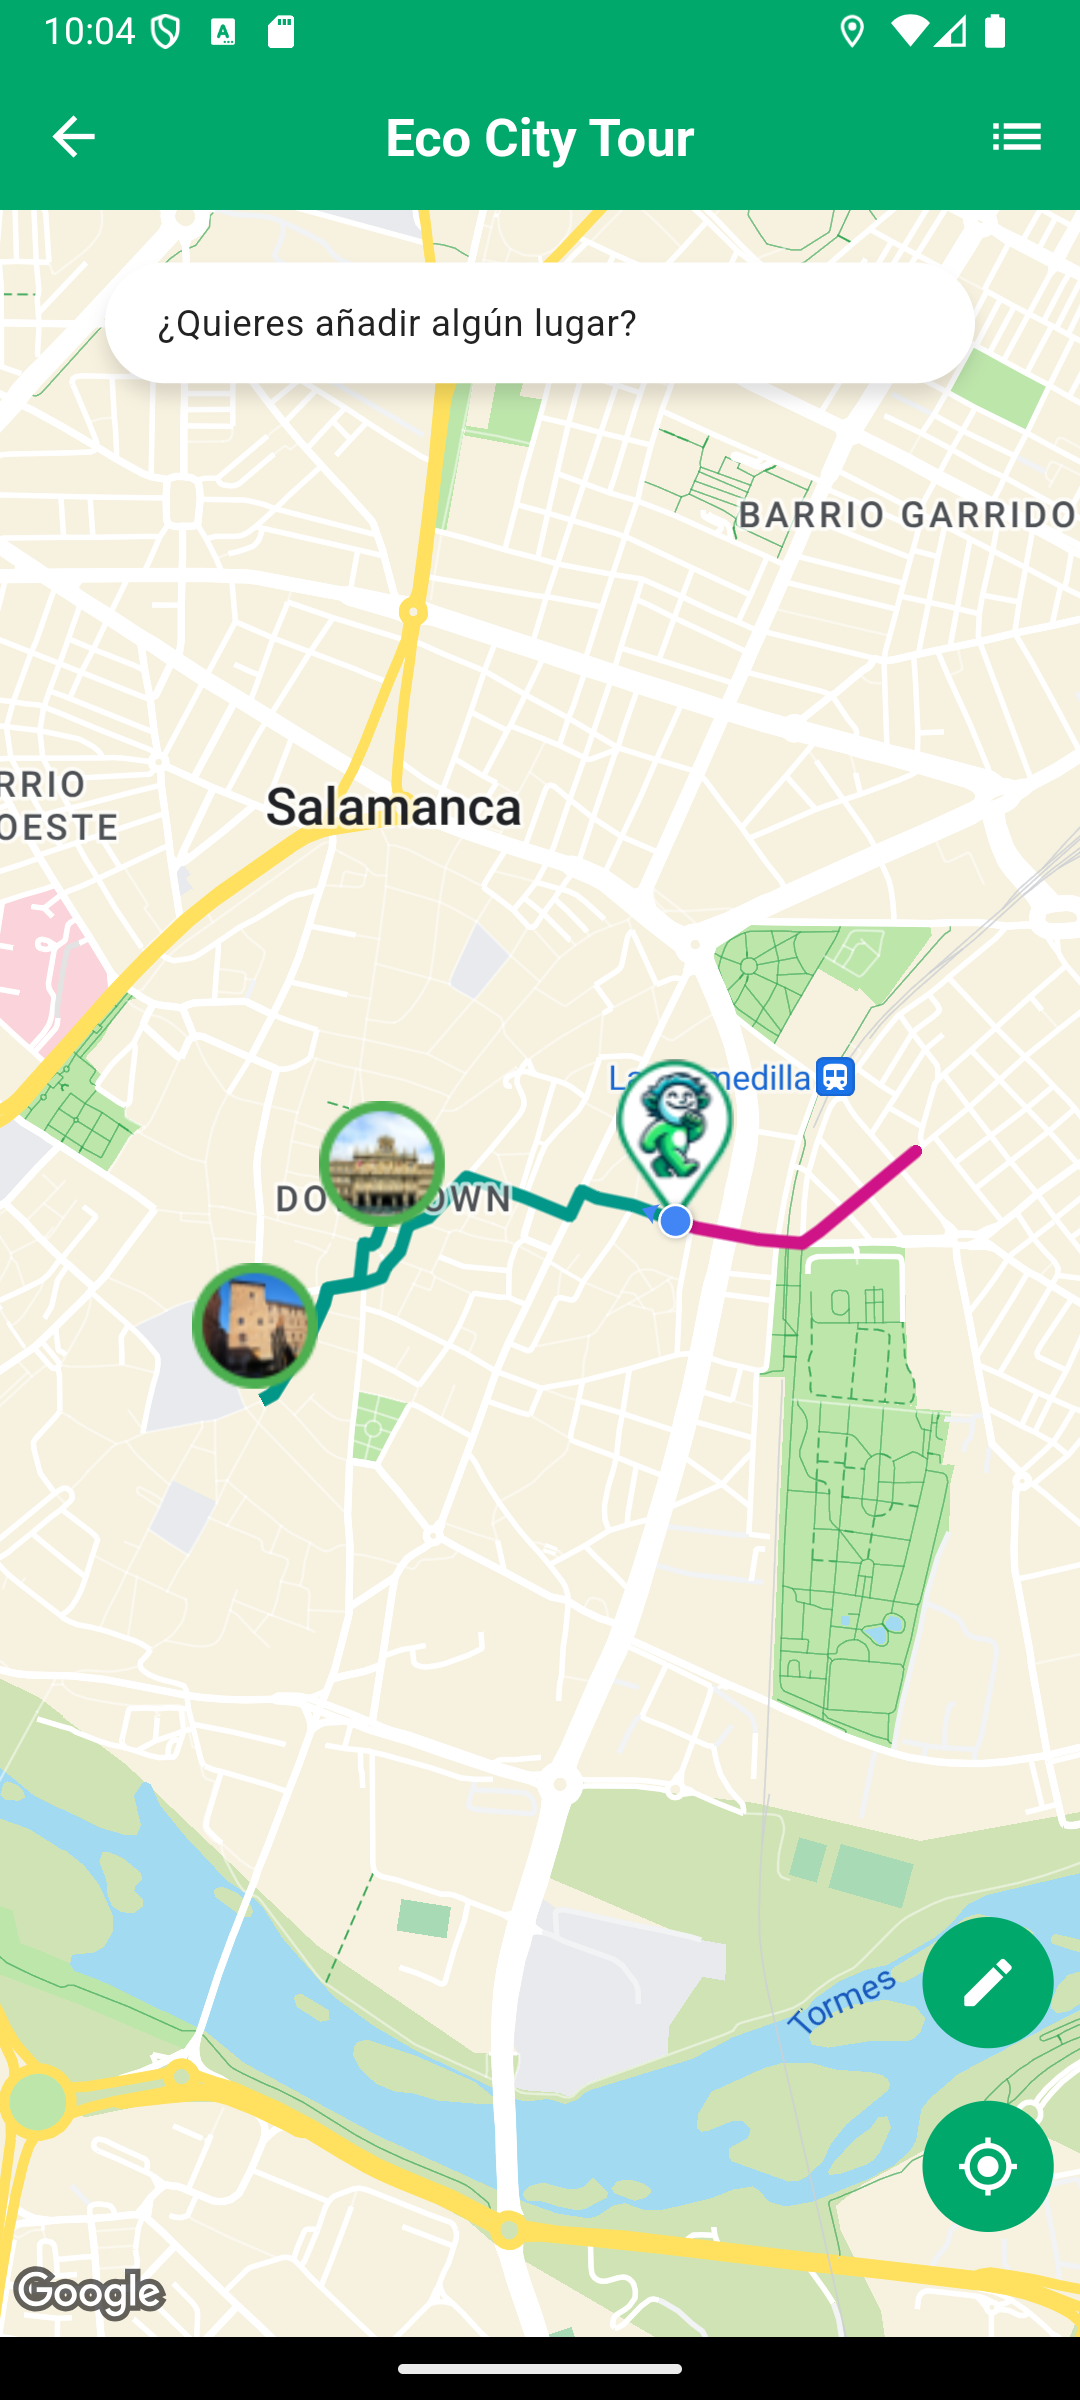
\includegraphics[width=0.6\linewidth]{E10-join-tour} & 
		\vspace{-10pt}
		
		La primera acción que debe realizar el usuario al iniciar la aplicación es habilitar el permiso de uso de GPS. Esto permite que la aplicación acceda a la ubicación del dispositivo para calcular rutas y mostrar información relevante.
		\textbf{Pasos a seguir:}
		\begin{enumerate}
			\item Al abrir la aplicación por primera vez, aparecerá la pantalla mostrada en la Figura~\ref{fig:joinECT}.
			\item Pulse el botón \textbf{Solicitar acceso al GPS}.
			\item Conceda el permiso solicitado en la ventana emergente.
		\end{enumerate}		
	\end{tabular}
	\caption{Unirse al Eco City Tour}
	\label{fig:joinECT}
\end{figure}